\documentclass[a4paper,14pt]{extreport}
\usepackage[utf8]{inputenc}
\usepackage[T2A]{fontenc}
\usepackage[russian]{babel}
\usepackage{eufrak}
% поля:
\usepackage[left=1cm, right=1cm, top=2cm, bottom=2cm]{geometry}
\linespread{1}
\usepackage{indentfirst} % отделять первую строку раздела абзацным отступом
\setlength\parindent{5ex}
\addto{\captionsrussian}{\renewcommand*{\contentsname}{Содержание}}
\usepackage[hidelinks]{hyperref} % гиперссылки в содержании
\usepackage{graphicx}
\usepackage{float}
\usepackage{amsmath}
\renewcommand*{\thesection}{\arabic{section}}

\usepackage{multirow}
\usepackage[normalem]{ulem}
\useunder{\uline}{\ul}{}

\usepackage{cmap}%позволяет копировать кириллицу из скомпилированного файла

% Глубина разделов, попадающих в содержание
\setcounter{tocdepth}{3}

\linespread{1.3} % настройка межстрочного интервала
\tolerance=1000 % настройка чувствительности вставки переносов
\hfuzz=0pt
\sloppy

\begin{document}
% Переменование "Список литературы" в "Литература"
\renewcommand{\refname}{Литература}
\begin{titlepage}
	\begin{center}
		\large
		МИНИСТЕРСТВО ОБРАЗОВАНИЯ И НАУКИ\\ РОССИЙСКОЙ ФЕДЕРАЦИИ
		
		\textbf{Федеральное агентство по образованию}
		\vspace{0.5cm}
		
		УНИВЕРСИТЕТ ИТМО
		\vspace{0.25cm}
		
		Факультет компьютерных технологий и управления
		
		Кафедра систем управления и информатики
		\vfill
		
		
		Студент: Артемов Кирилл\\
		группа P4135\\
		
		\textsc{\LARGE Домашнее задание № 2}\\[5mm]
		
		{\LARGE Вывод уравнений движения плоского двухзвенного маятника на основе метода Ньютона-Эйлера и численная реализация в рекуррентном виде}	\bigskip
		
	\end{center}
	\vfill
	
	\newlength{\ML}
	\settowidth{\ML}{«\underline{\hspace{0.7cm}}» \underline{\hspace{1cm}}}
	\hfill\begin{minipage}{0.4\textwidth}
		Преподаватель\\
		\underline{\hspace{\ML}} С.\,А.~Колюбин\\
		«\underline{\hspace{0.7cm}}» \underline{\hspace{2cm}} 2016 г.
	\end{minipage}%
	\bigskip
	
	\vfill
	
	\begin{center}
		Санкт-Петербург, 2016 г.
	\end{center}
\end{titlepage}

\tableofcontents
\newpage

\section{Задание}

\begin{enumerate}
	\item Вывести аналитически уравнения движения плоского двухзвенного маятника (рисунок 1) на основе метода Ньютона-Эйлера;
	\item Разработать программу, реализующую полученную динамическую
	модель робота для решения обратной задачи динамики (численная реализация уравнений Ньютона-Эйлера в рекуррентном виде).
\end{enumerate}

\begin{figure}[H]
	\center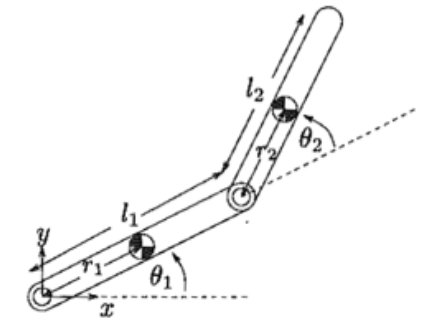
\includegraphics[width=0.5\linewidth]{images/1.png}
	\caption{Плоский двухзвенный маятник: 2 вращательных сочленения. Оба звена -- цилиндрические стержни.}
	\label{fig:scr1}
\end{figure}
На рисунке 1: $l_1, l_2$ -- длины звеньев, $r_1, r_2$ -- расстояния от начала звена до центра масс каждого из звеньев, $\theta_1, \theta_2$ -- углы поворота звеньев.


\section{Вывод уравнений движения}

\subsection{Инициализация}

Звенья вращательные, тогда пусть $q_i = \theta_i$.

Входные данные: $q, \dot q, \dot q$ -- траектория движения, $l_1, l_2, r_1, r_2, d^{link}_1,  d^{link}_2$ -- геометрические параметры, $m1, m2, I_i$ -- динамические параметры.

Первым делом прикрепим системы координат к маятнику в  с методом Денавита-Хартенберга как показано на рисунке 2.

\begin{figure}[H]
	\center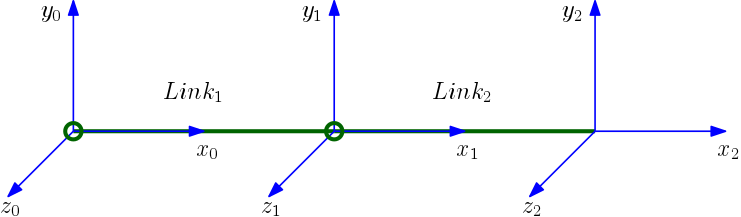
\includegraphics[width=0.8\linewidth]{images/2.png}
	\caption{Системы координат по методу ДХ}
	\label{fig:scr1}
\end{figure}

Составим таблицу 1 с параметрами ДХ.

\begin{table}[H]
	\centering
	\caption{Параметры ДХ}
	\label{my-label}
	\begin{tabular}{|c|l|l|l|l|}
		\hline
		№ & $a_i$ & $\alpha_i$ & $d_i$ & $\theta_i$ \\ \hline
		1 & $l_1$ & 0 & 0 & $q_1$ \\ \hline
		2 & $l_2$ & 0 & 0 & $q_2$ \\ \hline
	\end{tabular}
\end{table}

Матрицы поворота:

\begin{equation}
	^0R_1 =
	\begin{bmatrix}
		cos(q_1) & -sin(q_1) & 0\\
		sin(q_1)& cos(q_1) &0 \\
		0&0 &1
	\end{bmatrix}
\end{equation}

\begin{equation}
	^1R_2 =
	\begin{bmatrix}
	cos(q_2) & -sin(q_2) & 0\\
	sin(q_2)& cos(q_2) &0 \\
	0&0 &1
	\end{bmatrix}
\end{equation}


\subsection{Вывод уравнений}

\subsubsection{Расчет тензора инерции}

\begin{figure}[H]
	\center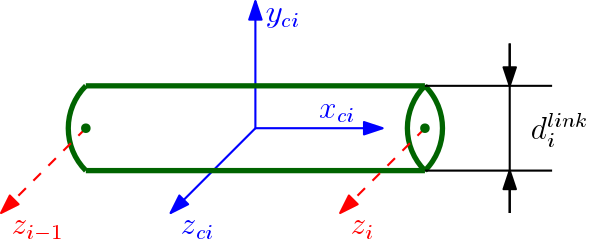
\includegraphics[width=0.8\linewidth]{images/3.png}
	\caption{Системы координат в звене}
	\label{fig:scr1}
\end{figure}
Примем за радиус $r_{li} = \frac{d^{link}_2}{2}$. Запишем моменты инерции для каждой из осей СК закрепленной в центре масс, как на рисунке 3. Для цилиндрического стержня это:
\begin{align}
	I_i^{xx} &= \frac{m_i r_{li}^2}{2} \\
	I_i^{yy} &= \frac{m_i (3 r_{li}^2 + l_i^2)}{12} \\
	I_i^{zz} &= \frac{m_i (3 r_{li}^2 + l_i^2)}{12}
\end{align}

Тензор инерции примет вид:
\begin{equation}
	I_i = 
	\begin{bmatrix}
	\frac{m_i r_{li}^2}{2} & 0 & 0 \\ 
	0 &    	\frac{m_i (3 r_{li}^2 + l_i^2)}{12} & 0\\
	0 & 0 & \frac{m_i (3 r_{li}^2 + l_i^2)}{12}
	\end{bmatrix}
\end{equation}

Так как ось вращения проходит через начало звена, а не через центр, то воспользовавшись теоремой Гюйгенса - Штейнера, получим тензор инерции относительно оси вращения звена. Формула для пересчета:

\begin{equation}
	J_{ij} = I_{ij} + m (\textbf{d}^2 * \delta_{ij} -d_i d_j)
\end{equation}
где $J_{ij}$ -- элемент полученного тензора, $I_{ij}$ -- элемент исходного тензора, $\textbf{d} = (d_1, d_2, d_3)$ -- вектор смещения центра масс ($r_1 = d_1, r_2 = d_1$ по оси $X$ для каждого звена из рисунка 1), $\delta_{ij}$ -- символ Кронекера.

Получаем тензор инерции для оси вращения звена (начало звена):
\begin{equation}
	J_i = 
\begin{bmatrix}
\frac{m_i r_{li}^2}{2} & 0 & 0 \\ 
0 &    \frac{m_i (3 r_{li}^2 + l_i^2)}{12} + m_i r_i^2 & 0\\
0 & 0 &\frac{m_i (3 r_{li}^2 + l_i^2)}{12} + m_i r_i^2
\end{bmatrix}
\end{equation}
где $r_i$ -- расстояние до центра масс звена $i$. Так как оба звена цилиндрические стержни, то полученный тензор инерции справедлив для обоих звеньев.

\subsubsection{Начальные условия}

\begin{align}
	n &= 2\\
	i &= 1..2\\
	g &= 9.82\\
	\omega_0 &= \dot \omega_0 =
	\begin{bmatrix}
		0&0&0
	\end{bmatrix}^T\\
	a_0 &=
	\begin{bmatrix}
0&g&0
\end{bmatrix}^T\\
	a_{c0} &=
	\begin{bmatrix}
0&0&0
\end{bmatrix}^T\\
	f_{3} &=
\begin{bmatrix}
0&0&0
\end{bmatrix}^T\\
	\tau_{3} &=
\begin{bmatrix}
0&0&0
\end{bmatrix}^T
\end{align}


\subsubsection{Уравнения для прямой рекурсии}
Далее, все векторы у которых нет верхнего левого индекса выражены в собственной системе координат каждого из звеньев.
\begin{itemize}
\item Звено 1

Запишем выражение для угловой скорости:
% \omega_1
\begin{align*}
\omega_1 = ^0R_1^T [\omega_0 + \dot q_1 z_0] =
\left[
\begin{matrix}\cos{\left (q_{1} \right )} & \sin{\left (q_{1} \right )} & 0\\- \sin{\left (q_{1} \right )} & \cos{\left (q_{1} \right )} & 0\\0 & 0 & 1
\end{matrix}
\right]
\left[\begin{matrix}0\\0\\\dot{q}_1\end{matrix}\right] = 
\left[\begin{matrix}0\\0\\\dot{q}_1\end{matrix}\right]
\end{align*}
Запишем выражение для углового ускорения:
% \dot \omega_1
\begin{align*}
\dot \omega_1 = ^0R_1^T [\dot \omega_0 + \ddot q_1 z_0 + \dot q_1 \omega_0 \times z_0] = 
\left[
\begin{matrix}\cos{\left (q_{1} \right )} & \sin{\left (q_{1} \right )} & 0\\- \sin{\left (q_{1} \right )} & \cos{\left (q_{1} \right )} & 0\\0 & 0 & 1
\end{matrix}
\right]
\left[\begin{matrix}0\\0\\\ddot{q}_1\end{matrix}\right]
=
\left[\begin{matrix}0\\0\\\ddot{q}_1\end{matrix}\right]
\end{align*}
Запишем выражение для линейного ускорения:
% a1
\begin{align*}
&a_1 = ^0R_1^T a_0 + \dot \omega_1 \times ^1r_{01} + \omega_1 \times (\omega_1 \times ^1r_{01})
=\\
&=
\left[\begin{matrix}g \sin{\left (q_{1} \right )}\\g \cos{\left (q_{1} \right )}\\0\end{matrix}\right]
+
\left[\begin{matrix}0\\\ddot{q}_1 l_{1}\\0\end{matrix}\right]
+
\left[\begin{matrix}- \dot{q}_1^{2} l_{1}\\0\\0\end{matrix}\right]
=
\left[\begin{matrix}- \dot{q}_1^{2} l_{1} + g \sin{\left (q_{1} \right )}\\\ddot{q}_1 l_{1} + g \cos{\left (q_{1} \right )}\\0\end{matrix}\right]
\end{align*}

Запишем выражение для линейного ускорения центра масс:
% ac1
\begin{align*}
&a_{c1} = a_1 + \dot \omega_1 \times r_{1,c1} + \omega_1 \times (\omega_1 \times r_{1,c1})
=\\
&=
\left[\begin{matrix}- \dot{q}_1^{2} l_{1} + g \sin{\left (q_{1} \right )}\\\ddot{q}_1 l_{1} + g \cos{\left (q_{1} \right )}\\0\end{matrix}\right]
+
\left[\begin{matrix}0\\\ddot{q}_1 \left(- l_{1} + r_{1}\right)\\0\end{matrix}\right]
+
\left[\begin{matrix}- \dot{q}_1^{2} \left(- l_{1} + r_{1}\right)\\0\\0\end{matrix}\right]
=\\
&=
\left[\begin{matrix}- \dot{q}_1^{2} l_{1} - \dot{q}_1^{2} \left(- l_{1} + r_{1}\right) + g \sin{\left (q_{1} \right )}\\\ddot{q}_1 l_{1} + \ddot{q}_1 \left(- l_{1} + r_{1}\right) + g \cos{\left (q_{1} \right )}\\0\end{matrix}\right]
\end{align*}

%*********************************
\item Звено 2

Запишем выражение для угловой скорости: 
% \omega_2
\begin{align*}
\omega_2 &= ^1R_2^T [\omega_1 + \dot q_2 z_1] = 
\left[\begin{matrix}\cos{\left (q_{2} \right )} & \sin{\left (q_{2} \right )} & 0\\- \sin{\left (q_{2} \right )} & \cos{\left (q_{2} \right )} & 0\\0 & 0 & 1\end{matrix}\right]
\left[\begin{matrix}0\\0\\\dot{q}_1 + \dot{q}_2\end{matrix}\right]
=
\left[\begin{matrix}0\\0\\\dot{q}_1 + \dot{q}_2\end{matrix}\right]
\end{align*}
Запишем выражение для углового ускорения:
% \dot \omega_2
\begin{align*}
\dot \omega_2 &= ^1R_2^T [\dot \omega_1 + \ddot q_2 z_1 + \dot q_2 \omega_1 \times z_1] 
=\\
&=
\left[\begin{matrix}\cos{\left (q_{2} \right )} & \sin{\left (q_{2} \right )} & 0\\- \sin{\left (q_{2} \right )} & \cos{\left (q_{2} \right )} & 0\\0 & 0 & 1\end{matrix}\right]
\left[\begin{matrix}0\\0\\\ddot{q}_1 + \ddot{q}_2\end{matrix}\right]
=
\left[\begin{matrix}0\\0\\\ddot{q}_1 + \ddot{q}_2\end{matrix}\right]
\end{align*}
Запишем выражение для линейного ускорения:
% a2
\begin{align*}
a_2 &= ^1R_2^T a_1 + \dot \omega_2 \times ^2r_{12} + \omega_2 \times (\omega_2 \times ^2r_{11}) = \\
&=
\left[\begin{matrix}\left(\ddot{q}_1 l_{1} + g \cos{\left (q_{1} \right )}\right) \sin{\left (q_{2} \right )} + \left(- \dot{q}_1^{2} l_{1} + g \sin{\left (q_{1} \right )}\right) \cos{\left (q_{2} \right )}\\\left(\ddot{q}_1 l_{1} + g \cos{\left (q_{1} \right )}\right) \cos{\left (q_{2} \right )} - \left(- \dot{q}_1^{2} l_{1} + g \sin{\left (q_{1} \right )}\right) \sin{\left (q_{2} \right )}\\0\end{matrix}\right]
+\\
&+
\left[\begin{matrix}0\\l_{2} \left(\ddot{q}_1 + \ddot{q}_2\right)\\0\end{matrix}\right]
+
\left[\begin{matrix}- l_{2} \left(\dot{q}_1 + \dot{q}_2\right)^{2}\\0\\0\end{matrix}\right]
=\\
&=
\left[\begin{matrix}- l_{2} \left(\dot{q}_1 + \dot{q}_2\right)^{2} + \left(\ddot{q}_1 l_{1} + g \cos{\left (q_{1} \right )}\right) \sin{\left (q_{2} \right )} + \left(- \dot{q}_1^{2} l_{1} + g \sin{\left (q_{1} \right )}\right) \cos{\left (q_{2} \right )}\\l_{2} \left(\ddot{q}_1 + \ddot{q}_2\right) + \left(\ddot{q}_1 l_{1} + g \cos{\left (q_{1} \right )}\right) \cos{\left (q_{2} \right )} - \left(- \dot{q}_1^{2} l_{1} + g \sin{\left (q_{1} \right )}\right) \sin{\left (q_{2} \right )}\\0\end{matrix}\right]
\end{align*}
Запишем выражение для линейного ускорения центра масс:
% ac2
\begin{align*}
a_{c2} &= a_2 + \dot \omega_2 \times r_{2,c2} + \omega_2 \times (\omega_2 \times r_{2,c2}) 
=\\
&=
\left[\begin{matrix}- l_{2} \left(\dot{q}_1 + \dot{q}_2\right)^{2} + \left(\ddot{q}_1 l_{1} + g \cos{\left (q_{1} \right )}\right) \sin{\left (q_{2} \right )} + \left(- \dot{q}_1^{2} l_{1} + g \sin{\left (q_{1} \right )}\right) \cos{\left (q_{2} \right )}\\l_{2} \left(\ddot{q}_1 + \ddot{q}_2\right) + \left(\ddot{q}_1 l_{1} + g \cos{\left (q_{1} \right )}\right) \cos{\left (q_{2} \right )} - \left(- \dot{q}_1^{2} l_{1} + g \sin{\left (q_{1} \right )}\right) \sin{\left (q_{2} \right )}\\0\end{matrix}\right]
=\\
&=
\left[\begin{matrix}0\\\left(\ddot{q}_1 + \ddot{q}_2\right) \left(- l_{2} + r_{2}\right)\\0\end{matrix}\right]
+
\left[\begin{matrix}- \left(\dot{q}_1 + \dot{q}_2\right)^{2} \left(- l_{2} + r_{2}\right)\\0\\0\end{matrix}\right]
=\\
&=
\left[\begin{matrix}
- l_{2} \left(\dot{q}_1 + \dot{q}_2\right)^{2} - \left(\dot{q}_1 + \dot{q}_2\right)^{2} \left(- l_{2} + r_{2}\right) + \left(\ddot{q}_1 l_{1} \right.+\\+\left. g \cos{\left (q_{1} \right )}\right) \sin{\left (q_{2} \right )} + \left(- \dot{q}_1^{2} l_{1} + g \sin{\left (q_{1} \right )}\right) \cos{\left (q_{2} \right )}\\
l_{2} \left(\ddot{q}_1 + \ddot{q}_2\right) + \left(\ddot{q}_1 + \ddot{q}_2\right) \left(- l_{2} + r_{2}\right) + \left(\ddot{q}_1 l_{1} \right.+\\+\left. g \cos{\left (q_{1} \right )}\right) \cos{\left (q_{2} \right )} - \left(- \dot{q}_1^{2} l_{1} + g \sin{\left (q_{1} \right )}\right) \sin{\left (q_{2} \right )}\\0\end{matrix}
\right]
\end{align*}
\end{itemize}


\subsubsection{Уравнения для обратной рекурсии}

%*********************************
%*********************************
\begin{itemize}
\item Звено 2

Запишем выражение для силы:
% f_2
\begin{align*}
f_2 &= f_3 + m_2 a_{c2} =\\
&=
\left[\begin{matrix}- m_{2} \left(- \ddot{q}_1 l_{1} \sin{\left (q_{2} \right )} + \dot{q}_1^{2} l_{1} \cos{\left (q_{2} \right )} + \dot{q}_1^{2} r_{2} + 2 \dot{q}_1 \dot{q}_2 r_{2} + \dot{q}_2^{2} r_{2} - g \sin{\left (q_{1} + q_{2} \right )}\right)\\m_{2} \left(\ddot{q}_1 l_{1} \cos{\left (q_{2} \right )} + \ddot{q}_1 r_{2} + \ddot{q}_2 r_{2} + \dot{q}_1^{2} l_{1} \sin{\left (q_{2} \right )} + g \cos{\left (q_{1} + q_{2} \right )}\right)\\0\end{matrix}\right]
\end{align*}
Запишем выражение для момента:
% \tau_2
\begin{align*}
\tau_2 &= \tau_3 - f_2 \times (^2 r_{12} + r_{2,c2}) + f_3 \times r_{2c2} + J_2 \dot \omega_2 + \omega_2 \times (J_2 \omega_2) =\\
&=
\left[\begin{matrix}0\\0\\0\end{matrix}\right]
+
\left[\begin{matrix}0\\0\\- m_{2} r_{2} \left(\ddot{q}_1 l_{1} \cos{\left (q_{2} \right )} + \ddot{q}_1 r_{2} + \ddot{q}_2 r_{2} + \dot{q}_1^{2} l_{1} \sin{\left (q_{2} \right )} + g \cos{\left (q_{1} + q_{2} \right )}\right)\end{matrix}\right]
+\\
&+
\left[\begin{matrix}0\\0\\0\end{matrix}\right]
+
\left[\begin{matrix}0\\0\\
\frac{1}{12} \left(\ddot{q}_1 + \ddot{q}_2\right) \left(12 m_{2} r^{l2}_{2} + \operatorname{m_{2}}{\left (2 l_{2} + 3 r^{l2}_{2} \right )}\right)\end{matrix}\right]
+
\left[\begin{matrix}0\\0\\0\end{matrix}\right]
=\\
&= 
\left[\begin{matrix}0\\0\\
m_{2} r_{2} \left(\ddot{q}_1 l_{1} \cos{\left (q_{2} \right )} + \ddot{q}_1 r_{2} + \ddot{q}_2 r_{2} + \dot{q}_1^{2} l_{1} \sin{\left (q_{2} \right )} + g \cos{\left (q_{1} + q_{2} \right )}\right) +\\ \frac{1}{12} \left(\ddot{q}_1 + \ddot{q}_2\right) \left(12 m_{2} r^{l2}_{2} + \operatorname{m_{2}}{\left (2 l_{2} + 3 r^{l2}_{2} \right )}\right)\end{matrix}\right]
\end{align*}

%**************************
\item Звено 1

Запишем выражение для силы:
% f_1
\begin{align*}
f_1 &= f_2 + m_1 a_{c1} =\\
&=
\left[
\begin{matrix}- m_{2} \left(- \ddot{q}_1 l_{1} \sin{\left (q_{2} \right )} + \dot{q}_1^{2} l_{1} \cos{\left (q_{2} \right )} + \dot{q}_1^{2} r_{2} + 2 \dot{q}_1 \dot{q}_2 r_{2} + \dot{q}_2^{2} r_{2} - g \sin{\left (q_{1} + q_{2} \right )}\right)\\
m_{2} \left(\ddot{q}_1 l_{1} \cos{\left (q_{2} \right )} + \ddot{q}_1 r_{2} + \ddot{q}_2 r_{2} + \dot{q}_1^{2} l_{1} \sin{\left (q_{2} \right )} + g \cos{\left (q_{1} + q_{2} \right )}\right)\\
0
\end{matrix}\right]
+\\
&+
\left[\begin{matrix}m_{1} \left(- \dot{q}_1^{2} r_{1} + g \sin{\left (q_{1} \right )}\right)\\
m_{1} \left(\ddot{q}_1 r_{1} + g \cos{\left (q_{1} \right )}\right)\\
0\end{matrix}\right]
=\\
&=
\left[\begin{matrix}
m_{1} \left(- \dot{q}_1^{2} r_{1} + g \sin{\left (q_{1} \right )}\right) - m_{2} \left(- \ddot{q}_1 l_{1} \sin{\left (q_{2} \right )} \right.+\\+\left. \dot{q}_1^{2} l_{1} \cos{\left (q_{2} \right )} + \dot{q}_1^{2} r_{2} + 2 \dot{q}_1 \dot{q}_2 r_{2} + \dot{q}_2^{2} r_{2} - g \sin{\left (q_{1} + q_{2} \right )}\right)\\
m_{1} \left(\ddot{q}_1 r_{1} + g \cos{\left (q_{1} \right )}\right) + m_{2} \left(\ddot{q}_1 l_{1} \cos{\left (q_{2} \right )} + \ddot{q}_1 r_{2} \right.+\\+\left. \ddot{q}_2 r_{2} + \dot{q}_1^{2} l_{1} \sin{\left (q_{2} \right )} + g \cos{\left (q_{1} + q_{2} \right )}\right)\\0\end{matrix}\right]
\end{align*}
Запишем выражение для момента:
% \tau_1
\begin{eqnarray}
\tau_1 = \tau_2 - f_1 \times (^1 r_{01} + r_{1,c1}) + f_2 \times r_{1c1} + J_1 \dot \omega_1 + \omega_1 \times (J_1 \omega_1) =\nonumber\\
=
\left[\begin{matrix}0\\0\\m_{2} r_{2} \left(\ddot{q}_1 l_{1} \cos{\left (q_{2} \right )} + \ddot{q}_1 r_{2} + \ddot{q}_2 r_{2} + \dot{q}_1^{2} l_{1} \sin{\left (q_{2} \right )} \right.+\\+\left. g \cos{\left (q_{1} + q_{2} \right )}\right) + \frac{1}{12} \left(\ddot{q}_1 + \ddot{q}_2\right) \left(12 m_{2} r_{l2}^{2} + \operatorname{m_{2}}{\left (2 l_{2} + 3 r_{l2}^{2} \right )}\right)\end{matrix}\right]
-\nonumber\\
-
\left[\begin{matrix}0\\0\\
- r_{1} \left(m_{1} \left(\ddot{q}_1 r_{1} + g \cos{\left (q_{1} \right )}\right) + m_{2} \left(\ddot{q}_1 l_{1} \cos{\left (q_{2} \right )} \right.\right. +\\+\left.\left. \ddot{q}_1 r_{2} + \ddot{q}_2 r_{2} + \dot{q}_1^{2} l_{1} \sin{\left (q_{2} \right )} + g \cos{\left (q_{1} + q_{2} \right )}\right)\right)\end{matrix}\right]
+\nonumber\\
+
\left[\begin{matrix}0\\0\\m_{2} \left(l_{1} - r_{1}\right) \left(\ddot{q}_1 l_{1} \cos{\left (q_{2} \right )} + \ddot{q}_1 r_{2} + \ddot{q}_2 r_{2} + \dot{q}_1^{2} l_{1} \sin{\left (q_{2} \right )} + g \cos{\left (q_{1} + q_{2} \right )}\right)\end{matrix}\right]
+\nonumber\\
+
\left[\begin{matrix}0\\0\\\frac{\ddot{q}_1}{12} \left(12 m_{1} r_{l1}^{2} + \operatorname{m_{1}}{\left (l_{1}^{2} + 3 r_{l1}^{2} \right )}\right)\end{matrix}\right]
+
\left[\begin{matrix}0\\0\\0\end{matrix}\right]
=\nonumber\\
=
\left[\begin{matrix}0\\0\\
\ddot{q}_1 l_{1}^{2} m_{2} \cos{\left (q_{2} \right )} + \ddot{q}_1 l_{1} m_{2} r_{2} \cos{\left (q_{2} \right )} + \ddot{q}_1 l_{1} m_{2} r_{2} + \ddot{q}_1 m_{1} r_{1}^{2} +\\+
\ddot{q}_1 m_{1} r_{l1}^{2} + \ddot{q}_1 m_{2} r_{2}^{2} + \ddot{q}_1 m_{2} r_{l2}^{2} + \frac{\ddot{q}_1}{12} \operatorname{m_{1}}{\left (l_{1}^{2} + 3 r_{l1}^{2} \right )} +\\+ \frac{\ddot{q}_1}{12} \operatorname{m_{2}}{\left (2 l_{2} + 3 r_{l2}^{2} \right )} + \ddot{q}_2 l_{1} m_{2} r_{2} +\\+
\ddot{q}_2 m_{2} r_{2}^{2} + \ddot{q}_2 m_{2} r_{l2}^{2} + \frac{\ddot{q}_2}{12} \operatorname{m_{2}}{\left (2 l_{2} + 3 r_{l2}^{2} \right )} +\\+
\dot{q}_1^{2} l_{1}^{2} m_{2} \sin{\left (q_{2} \right )} + \dot{q}_1^{2} l_{1} m_{2} r_{2} \sin{\left (q_{2} \right )} +\\+ g l_{1} m_{2} \cos{\left (q_{1} + q_{2} \right )} + g m_{1} r_{1} \cos{\left (q_{1} \right )} + g m_{2} r_{2} \cos{\left (q_{1} + q_{2} \right )}
\end{matrix}\right]\nonumber
\end{eqnarray}
\end{itemize}

\subsubsection{Уравнения движения}

Так как звенья рассматриваемого плоского маятника вращательные, то необходимо произвести проекцию моментов на оси их вращения. 

\begin{eqnarray}
u_{1} = \tau_{1}^{T} z_{0} = \ddot{q}_1 l_{1}^{2} m_{2} \cos{\left (q_{2} \right )}
+ \ddot{q}_1 l_{1} m_{2} r_{2} \cos{\left (q_{2} \right )} + \ddot{q}_1 l_{1} m_{2} r_{2} +\nonumber\\
+ \ddot{q}_1 m_{1} r_{1}^{2} + \ddot{q}_1 m_{1} r_{l1}^{2} + \ddot{q}_1 m_{2} r_{2}^{2}
+ \ddot{q}_1 m_{2} r_{l2}^{2} + \frac{\ddot{q}_1}{12} \operatorname{m_{1}}{\left (l_{1}^{2} + 3 r_{l1}^{2} \right )} +\nonumber\\
+ \frac{\ddot{q}_1}{12} \operatorname{m_{2}}{\left (2 l_{2} + 3 r_{l2}^{2} \right )} + \ddot{q}_2 l_{1} m_{2} r_{2} + \ddot{q}_2 m_{2} r_{2}^{2} + \ddot{q}_2 m_{2} r_{l2}^{2} +\nonumber\\
+ \frac{\ddot{q}_2}{12} \operatorname{m_{2}}{\left (2 l_{2} + 3 r_{l2}^{2} \right )}
+ \dot{q}_1^{2} l_{1}^{2} m_{2} \sin{\left (q_{2} \right )} + \dot{q}_1^{2} l_{1} m_{2} r_{2} \sin{\left (q_{2} \right )} +\nonumber\\
+ g l_{1} m_{2} \cos{\left (q_{1} + q_{2} \right )} + g m_{1} r_{1} \cos{\left (q_{1} \right )} + g m_{2} r_{2} \cos{\left (q_{1} + q_{2} \right )} \nonumber
\end{eqnarray}
\begin{eqnarray}
u_{2} = \tau_{2}^{T} z_{1} = m_{2} r_{2} \left(\ddot{q}_1 l_{1} \cos{\left (q_{2} \right )} + \ddot{q}_1 r_{2} + \ddot{q}_2 r_{2} + \dot{q}_1^{2} l_{1} \sin{\left (q_{2} \right )} + g \cos{\left (q_{1} + q_{2} \right )}\right) +\nonumber\\
+ \frac{1}{12} \left(\ddot{q}_1 + \ddot{q}_2\right) \left(12 m_{2} r_{l2}^{2} + \operatorname{m_{2}}{\left (2 l_{2} + 3 r_{l2}^{2} \right )}\right) \nonumber
\end{eqnarray}

Сгруппировав, получим окончательные уравнения движения плоского двухзвенного маятника:
\begin{eqnarray}
\left( l_{1}^{2} m_{2} \cos{\left (q_{2} \right )}
+ l_{1} m_{2} r_{2} \cos{\left (q_{2} \right )} + l_{1} m_{2} r_{2} + m_{1} r_{1}^{2} + m_{1} r_{l1}^{2} +  m_{2} r_{2}^{2} +  m_{2} r_{l2}^{2} +\nonumber\right.\\\left. 
+ \frac{1}{12} \operatorname{m_{1}}{\left (l_{1}^{2} + 3 r_{l1}^{2} \right )} + \frac{1}{12} \operatorname{m_{2}}{\left (2 l_{2} + 3 r_{l2}^{2} \right )} + 
\right) \ddot{q}_1 +\nonumber\\+
\left(
 l_{1} m_{2} r_{2} +  m_{2} r_{2}^{2} +  m_{2} r_{l2}^{2} + \frac{1}{12} \operatorname{m_{2}}{\left (2 l_{2} + 3 r_{l2}^{2} \right )}
+ \right) \ddot{q}_2 +\nonumber\\+
\left(
l_{1}^{2} m_{2} \sin{\left (q_{2} \right )}  + l_{1} m_{2} r_{2} \sin{\left (q_{2} \right )} 
\right)\dot{q}_1^{2} +\nonumber\\
+ g l_{1} m_{2} \cos{\left (q_{1} + q_{2} \right )} + g m_{1} r_{1} \cos{\left (q_{1} \right )} + g m_{2} r_{2} \cos{\left (q_{1} + q_{2} \right )} = u_{1}\nonumber
\end{eqnarray}
\begin{eqnarray}
\left(m_{2} r_{l2}^{2} + \frac{1}{12} \operatorname{m_{2}}{\left (2 l_{2} + 3 r_{l2}^{2} \right )}\right) \left(\ddot{q}_1 + \ddot{q}_2\right) + \nonumber \\
+\left(m_{2} r_{2} l_{1} \cos{\left (q_{2} \right )} + m_{2} r_{2} r_{2}\right)
\ddot{q}_1 + \nonumber \\
 + m_{2} r_{2}  r_{2} \ddot{q}_2 + \nonumber \\
 + m_{2} r_{2} l_{1} \sin{\left (q_{2} \right )} \dot{q}_1^{2} +\nonumber\\
+ m_{2} r_{2} g \cos{\left (q_{1} + q_{2} \right )} = u_{2}\nonumber
\end{eqnarray}

\newpage
\section{Расчет траектории}

Для моделирования численного алгоритма, на вход которого нужно подавать траекторию движения, рассчитаем ее методом сплайн-функций.

Для упрощения расчетов воспользуемся нормированным временем $t \in [0, 1]$.

\begin{center}
	$t = \frac{\tau - \tau_{i-1}}{\tau_{i} - \tau_{i-1}};$
	$\tau \in [\tau_{i-1}, \tau_{i}]; t \in [0, 1]$	
	\\
\end{center}

Траектория для звена $i$ представляет собой три полинома:
\begin{equation*}
\begin{cases}
q_i(t) = a_0 + a_1  t + a_2  t^2 + a_3 t^3 + a_4 t^4 + a_5 t^5\\
\dot q_i(t) = a_1 + 2 a_2  t + 3 a_3 t^2 + 4 a_4 t^3 + 5 a_5 t^4\\
\ddot q_i(t) = 2 a_2 + 6 a_3 t + 12 a_4 t^2 + 20 a_5 t^2\\
\end{cases}
\end{equation*}

Начальные и конечные значения для траектории представлены в таблице 1. 

\begin{table}[H]
	\centering
	\caption{Граничные условия траектории}
	\label{my-label}
	\begin{tabular}{|c|c|}
		\hline
		Начало         & Конец          \\ \hline
		$q_i(0) = q_s$    & $q_i(1) = q_e $   \\ \hline
		$	\dot q_i(0) = dq_s $ &$ \dot q_i(1) = dq_e $ \\ \hline
		$	\ddot q_i(0) = ddq_s$ & $\ddot q_i(1) = ddq_e$ \\ \hline
	\end{tabular}
\end{table}


Далее, запишем шесть уравнений, необходимых для нахождения неизвестных коэффициентов полиномов:
\begin{align*}
a_0&= q_{is}\\
a_1&= dq_{is}\\
2 a_2&= ddq_{is}\\
a_0 + a_1 + a2 + a3 + a4 + a5 &= q_{ie}\\
a_1 + 2 a2 + 3 a3 + 4 a4 + 5 a5&= dq_{ie}\\
2 a2 + 6 a3 + 12 a4 + 20 a5&= ddq_{ie}\\
\end{align*}

Упростив:
\begin{align*}
a3 + a4 + a5 &= q_{ie} - q_{is} - dq_{is} - \frac{1}{2} ddq_{is}\\
3 a3 + 4 a4 + 5 a5&= dq_{ie} - q_{is} - ddq_{is}\\
6 a3 + 12 a4 + 20 a5&= ddq_{ie} = ddq_{is}\\
\end{align*}

Получим матричное уравнение (полученные матрицы расположены не в модуле $init.py$, а непосредственно в $trajectory.py$):
\begin{align*}
\begin{bmatrix}
1&1&1\\
3&4&5\\
6& 12& 20
\end{bmatrix}
\begin{bmatrix}
a_3\\
a_4\\
a_5
\end{bmatrix}
=
\begin{bmatrix}
q_{ie} - q_{is} - dq_{is} - \frac{1}{2} ddq_{is}\\
dq_{ie} - q_{is} - ddq_{is}\\
ddq_{ie} = ddq_{is}\\
\end{bmatrix}
\end{align*}
Откуда найдем неизвестные коэффициенты:
\begin{align*}
\begin{bmatrix}
a_3\\
a_4\\
a_5
\end{bmatrix}
=
\begin{bmatrix}
1&1&1\\
3&4&5\\
6& 12& 20
\end{bmatrix}^{-1}
\begin{bmatrix}
q_{ie} - q_{is} - dq_{is} - \frac{1}{2} ddq_{is}\\
dq_{ie} - q_{is} - ddq_{is}\\
ddq_{ie} = ddq_{is}\\
\end{bmatrix}
\end{align*}

И наконец, задаем время движения манипулятора между точками и вычисляем для заданных интервалов времени значения полиномов.


\section{Численная реализация в рекуррентном виде}

Программа представляет из себя несколько модулей написанных на языке программирования Python. Список разработанных модулей:
\begin{enumerate}
\item $init.py$ -- содержит параметры, необходимые для расчета динамики робота, а также параметры траектории.
\item $task.py$ -- содержит функцию $main$, которая рассчитывает траекторию для заданных граничных условий в модуле $init.py$, строит ее график, а также для всех звеньев вычисляет:
\begin{enumerate}
	\item полную динамику;
	\item вектор гравитации;
	\item Кориолисовы/центробежные силы;
	\item матрицу инерции;
	\item обобщенные моменты.
\end{enumerate}
и строит графики зависимости вычисленных данных от времени.
\item $Kinematics.py$ -- содержит класс $Kinematics$ отвечающий за кинематику маятника, решение прямой и обратной задач кинематики. Был реализован в рамках курса лабораторных работ $Control Methots for Robotics$.
Для инициализации экземпляра класса в конструктор передаются массивы $a, \alpha, d, \theta$ -- параметры ДХ.
\item $Dynamics.py$ содержит функции расчета тензоров инерции $j = J(I_c, m, d)$, матриц трансформации $h = H(kinematicsObject, q, from, to)$, матриц поворота $r = R(kinematicsObject, q, from, to)$ и функцию решения обратной задачи динамики $u = NE(q,\dot q, \ddot q, kinematicsObject, g)$.
\item $trajectory.py$ содержит функции построения траектории движения для заданных начальных условий $q, \dot q, \ddot q = getTrajectories(initQ, initDQ, initDDQ, interval)$, где $initQ$ массив $n \times 2$ -- каждая строка содержит начальное и конечное значение обобщенной координаты. Тоже и для $initDQ, initDDQ$. $interval = [time_{start}, time_{end}, step]$.
\item $transformations.py$ -- содержит несколько функция для удобной работы с матрицами однородных преобразований.
\item $graphics.py$ -- содержит функции для построения графиков.
\end{enumerate}

На рисунках ниже изображены результаты работы программы.

\begin{figure}[]
	\center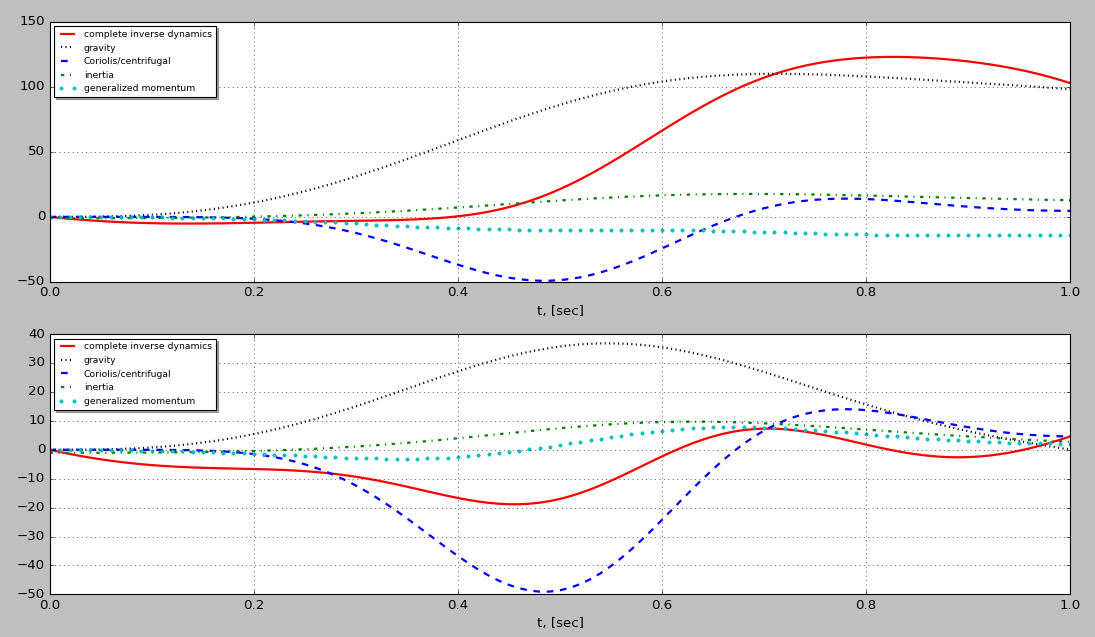
\includegraphics[width=0.9\linewidth]{images/4.png}
	\caption{Результаты выполнения задания}
	\label{fig:scr1}
\end{figure}

\begin{figure}[H]
	\center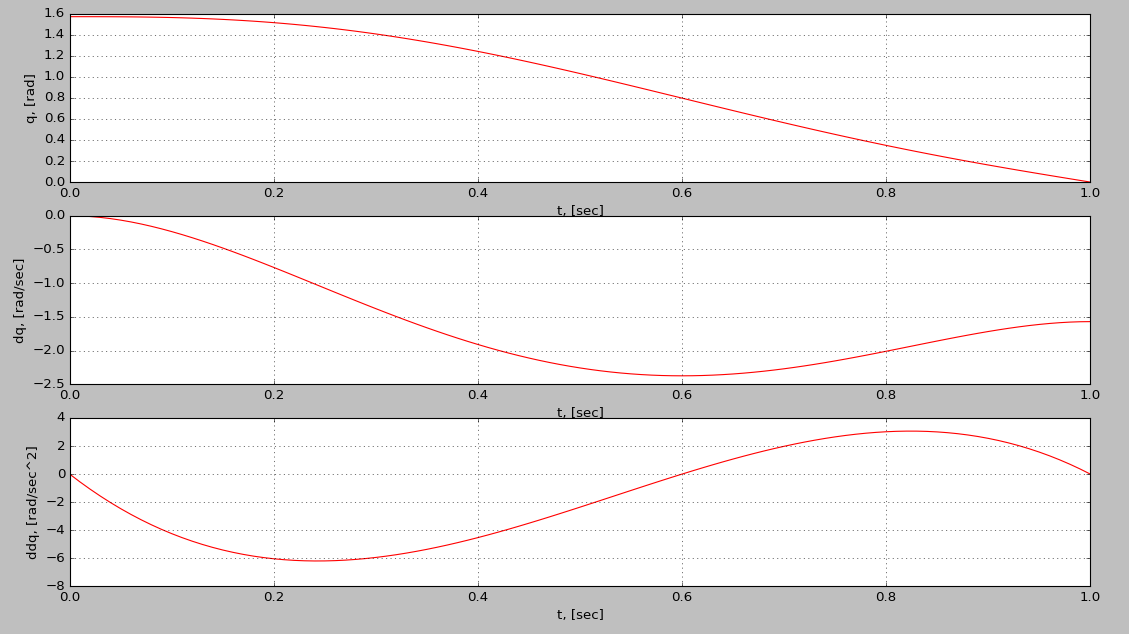
\includegraphics[width=0.9\linewidth]{images/q1.png}
	\caption{Траектория для звена 1}
	\label{fig:scr1}
\end{figure}


\begin{figure}[H]
	\center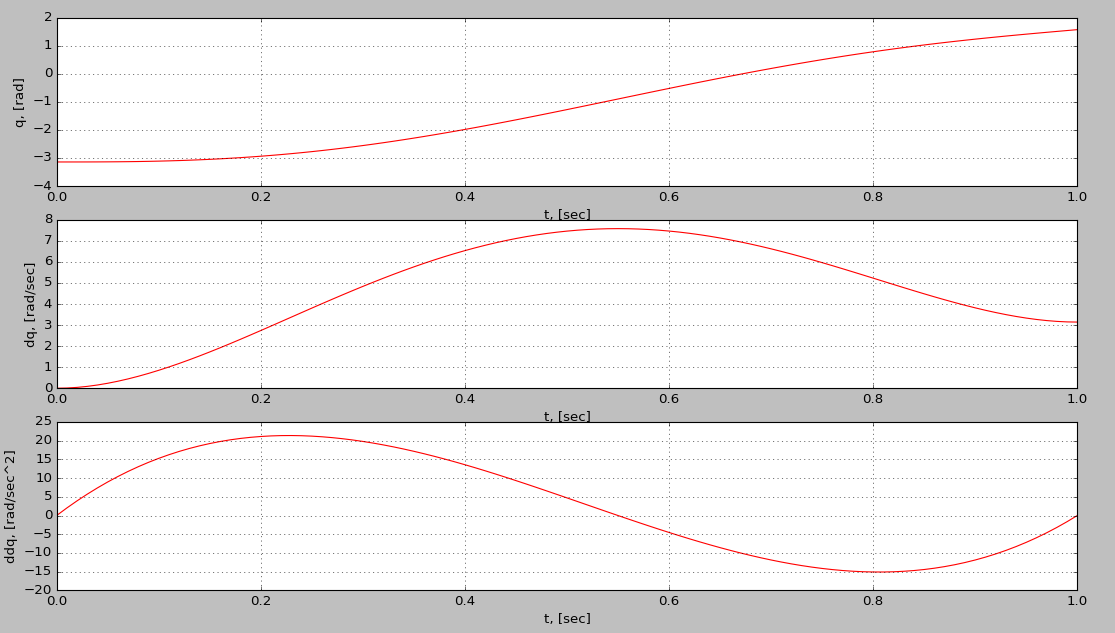
\includegraphics[width=0.9\linewidth]{images/q2.png}
	\caption{Траектория для звена 2}
	\label{fig:scr1}
\end{figure}



\section{Вывод}

В этой работе были получены уравнения движения для плоского двухзвенного маятника методом Ньютона-Эйлера, а также реализовано численное вычисление динамики для заданной траектории движения.

Следует отметить, что аналитический вывод уравнений методом Ньютона-Эйлера весьма сложен и уравнения получаются достаточно громоздкими, что бы допустить в них внушительное количество ошибок, в то время как численная реализация в программе укладывается в два десятка строк кода.

\end{document}


